\documentclass[10pt,twocolumn,a4j]{jarticle}
\usepackage{bm}
\usepackage{siunitx}
\usepackage{cases}
\usepackage[japanese]{babel}
\usepackage[dvipdfmx]{graphicx}
\usepackage{subfig}
\columnsep 3zw
\usepackage[dvipdfmx]{graphicx}
\usepackage{subfig} 
\title{A~Computational~Model~of~Cell~Migration~of~Fish~Keratocytes}
\author{生体情報システム研究~~徳永~優}
\date{}
\begin{document}
\maketitle
\section{はじめに}
\begin{figure}[tbp]
\centering
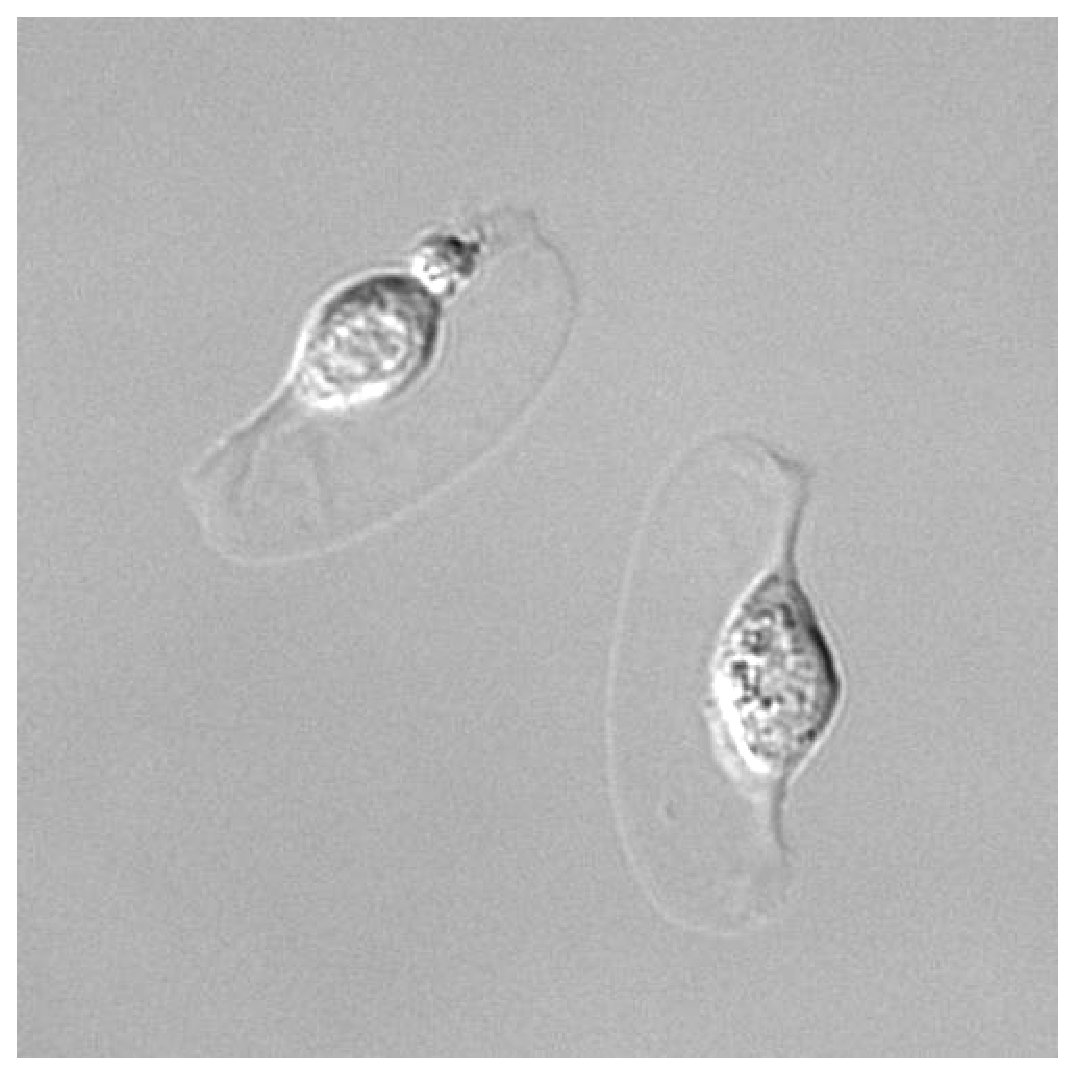
\includegraphics[scale=0.4]{kera.eps}
\caption{細胞遊走中のケラトサイト。(撮影:中田多可子氏(岩楯研究室))}
\label{fig:kera}
\end{figure}
魚類表皮細胞ケラトサイトは通常時に円形状の形態だが、細胞遊走を始めるときに半月状の形態に変形する(図\ref{fig:kera})。さらに、細胞遊走中はその半月状形態が維持される。この現象は、細胞の変形がケラトサイトの細胞遊走を実現するために重要な特徴であることを示唆している。しかし、半月状形態がどのように形成され、維持されるのかは明らかになっていない。本研究の目的は、ケラトサイトが半月状形態を形成、維持する細胞内メカニズムを細胞内メカニズムを考慮した物理シミュレーション実験により解明する。
\section{ケラトサイトの細胞遊走}
先行研究では、細胞骨格であるアクチン分子が重合してF-actinを形成することによって細胞膜へ伸長することが報告されており、これが細胞膜の変形および細胞の推進力の原因として示唆されてきた\cite{svitkina1997analysis}。アクチン分子の重合には極性があり、F-actinの一定の端でしか起こらない。アクチン分子は、細胞の前方に多く集中しており、アクチン分子濃度が高い場所であるほど重合の効率が良いこともわかっている。重合が起こらない端では逆に、F-actinからアクチン分子が解離していく脱重合という現象が起こっている。また、細胞後部の左右に広がるストレスファイバーと呼ばれる部位がアクチン分子を引き戻すアクチンレトログレードフロー(ARF)も報告されている\cite{swaminathan2017actin}。ARFに関して、ストレスファイバーの方向へアクチン分子が引き戻される時に、アクチン分子の重合方向が調整される配向効果も報告されている。つまり、細胞遊走中のアクチン分子は、細胞膜を押すために重合と脱重合を繰り返して伸長しているが、ARFによって細胞後方へ引き戻されているということになる。
\section{シミュレーション手法}
\begin{figure}[tbp]
\centering
 \subfloat[]{%
  \begin{tabular}{c}
   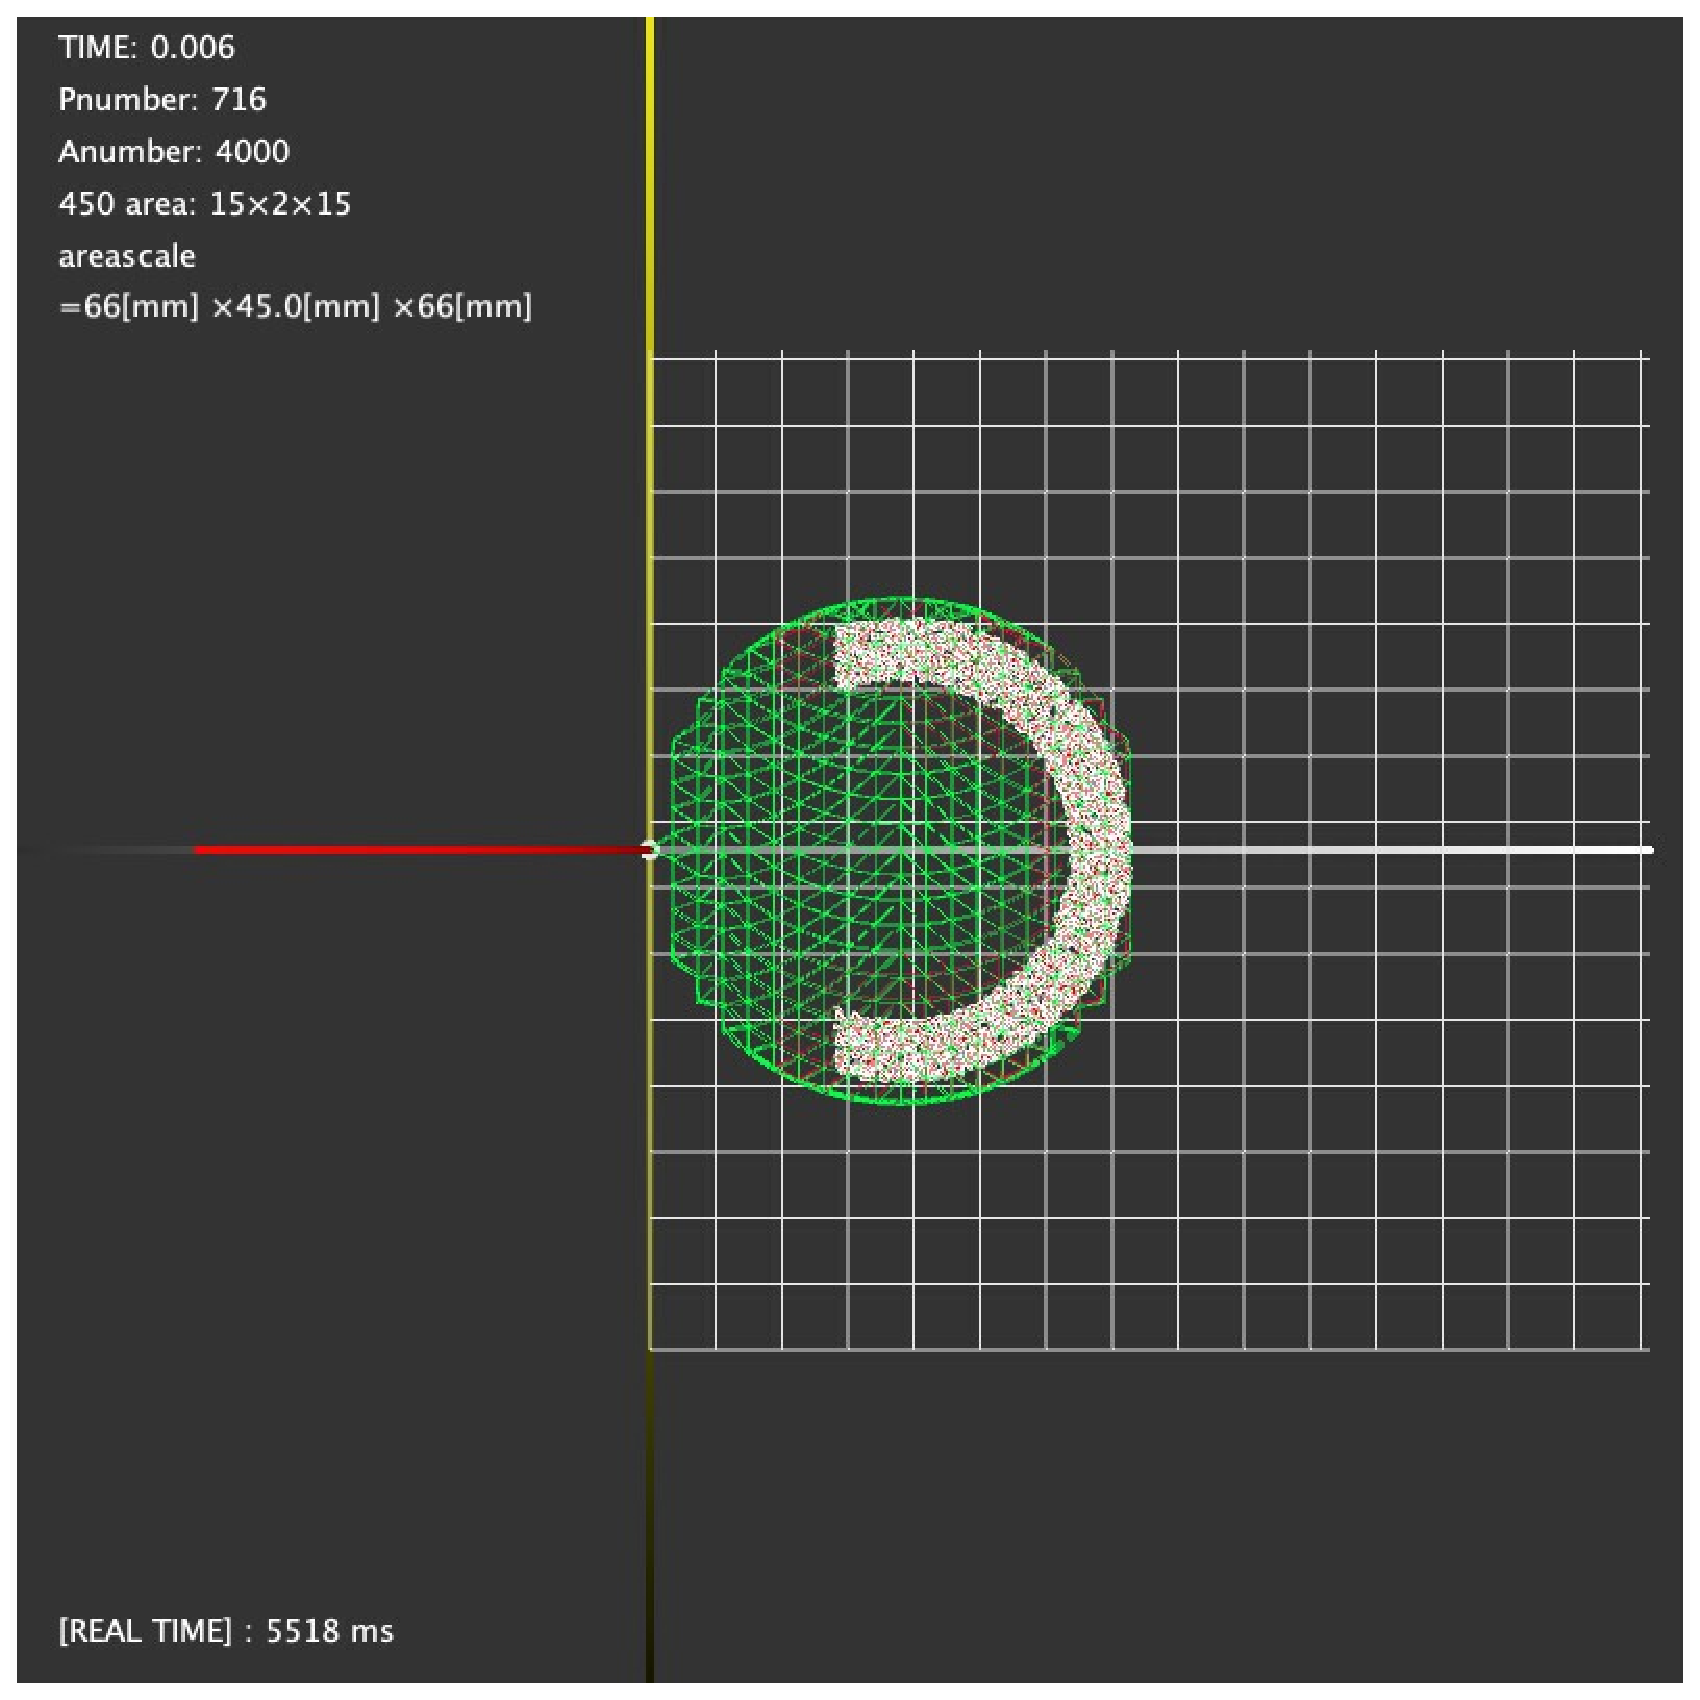
\includegraphics[width=4cm]{top.eps} 
  \end{tabular}
 }%
 \subfloat[]{%
  \begin{tabular}{c}
   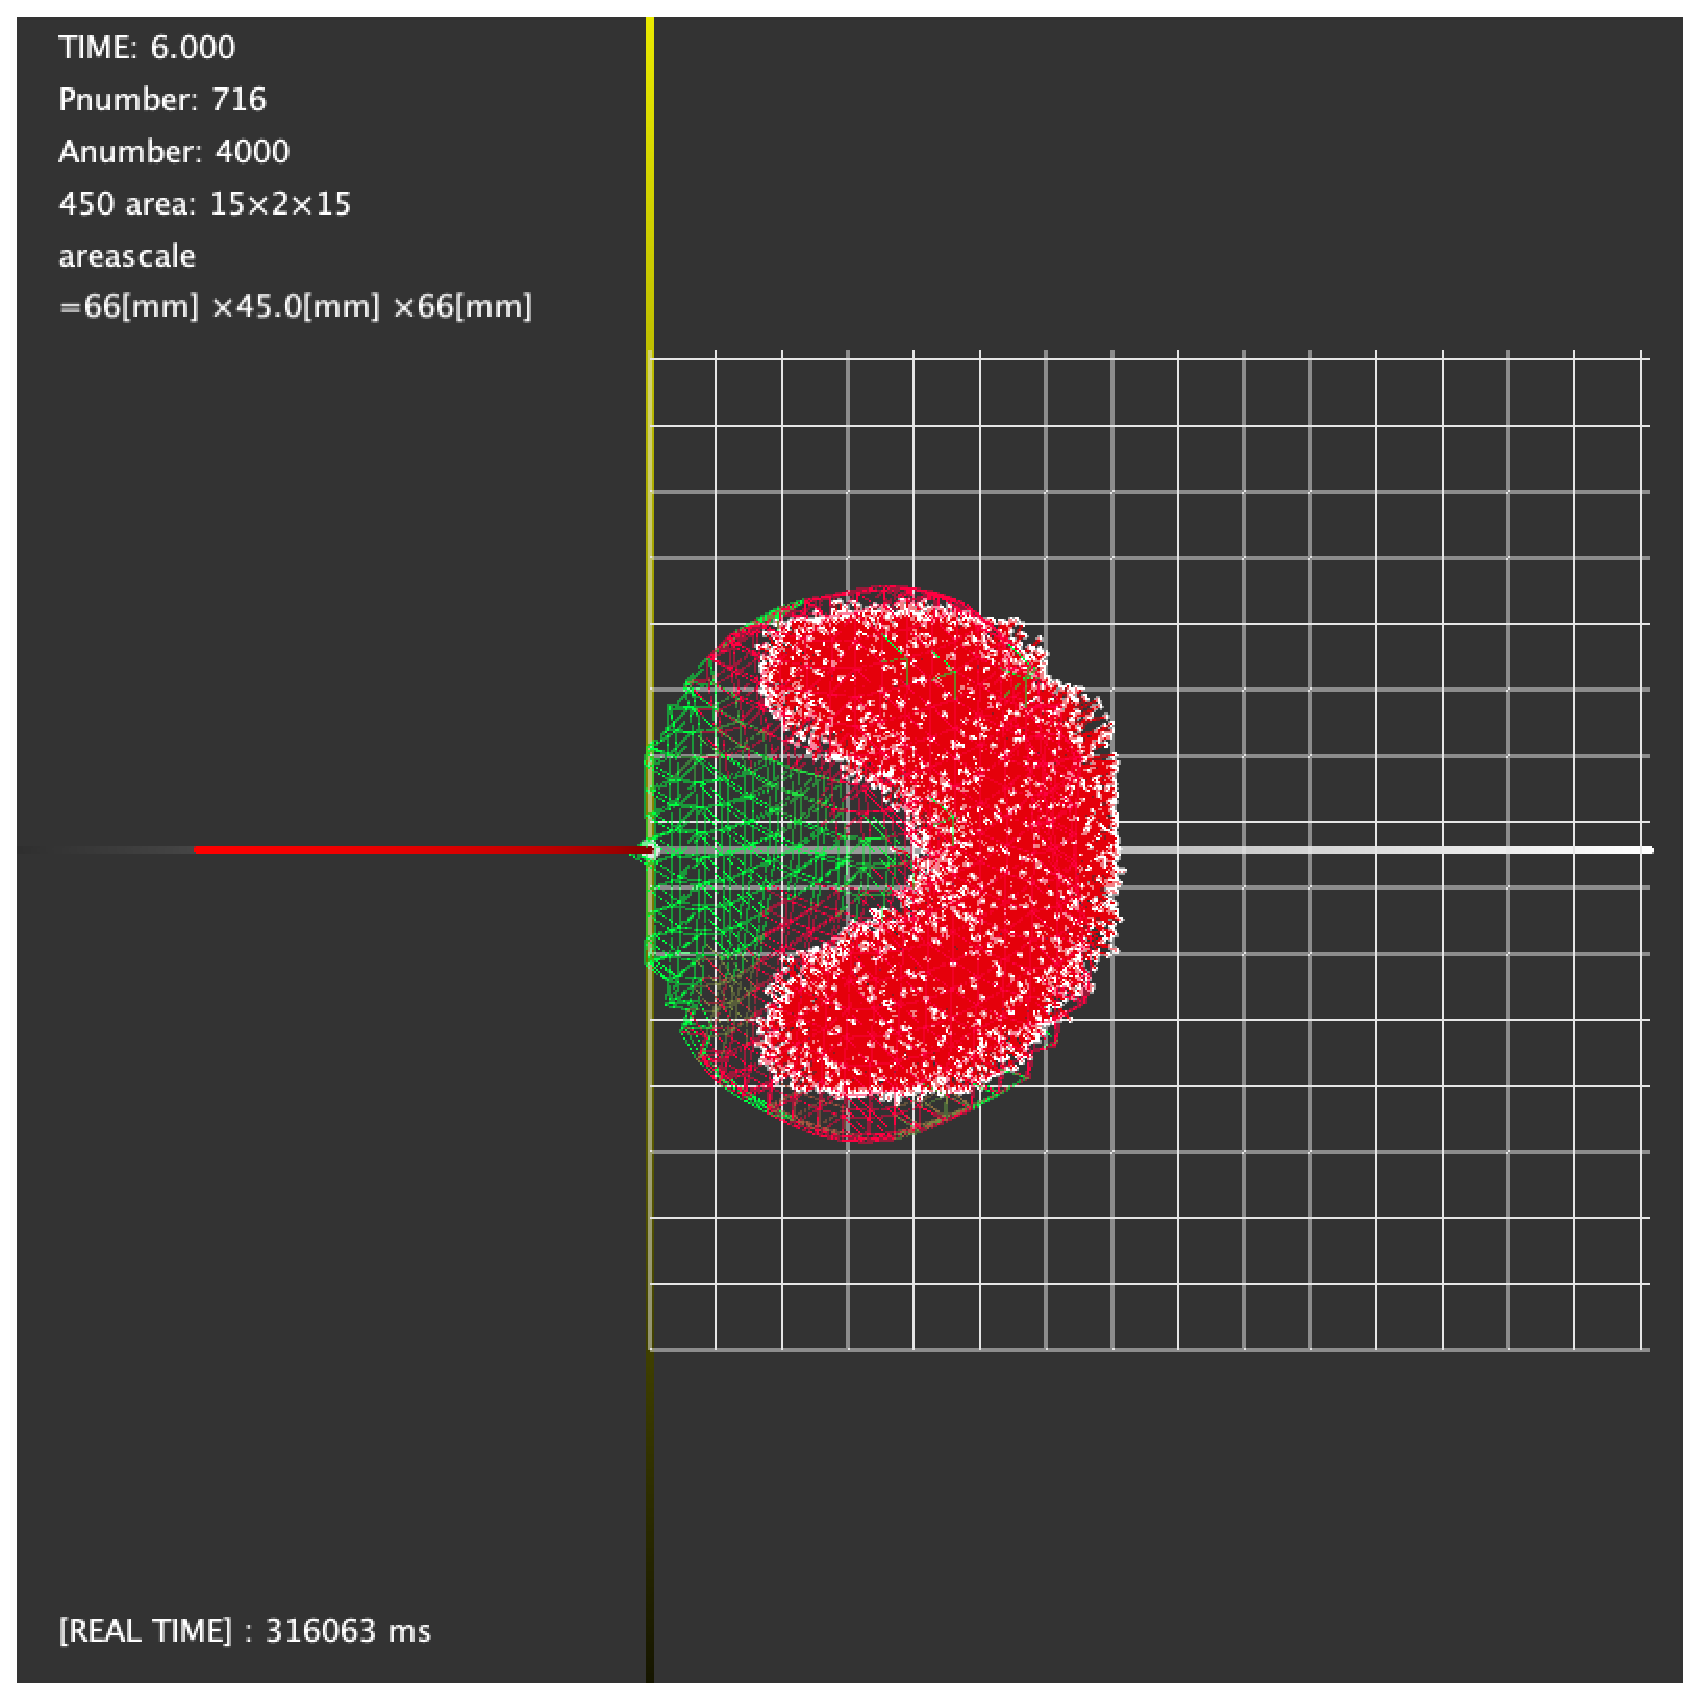
\includegraphics[width=4cm]{top60_arf.eps} 
  \end{tabular}
 }%
 \caption{シミュレーション結果。緑は細胞膜、白は重合前のアクチン分子、赤は重合後のF-actinを示す。}
 \label{fig:res0}
\end{figure}
本研究のシミュレーションでは、細胞膜は互いに相互作用する単純な粒子のネットワークによってモデル化され、初期条件として円柱形の表面に置かれた。各細胞膜分子$i$は、隣接する分子から弾性力$\bm{F}_i^m$を受け、重合によって近づいてきたアクチン分子から反発力$\bm{F}_i^a$を受けると仮定した(次式)。
\begin{equation}
m\frac{d^2\bm{x}_i}{dt^2} = \bm{F}^m_i +  \bm{F}^a_i - \eta \frac{d\bm{x}_i}{dt}
\end{equation}
ここで、$\bm{x}_i$は膜分子の位置、$\eta$は速度に比例する抵抗力の係数である。

また、アクチン分子は単純な棒によってモデル化され、重合および解重合はそれぞれ棒の一端の確率的伸びおよび他端の収縮によって表現した。初期条件として、アクチン分子は長さがなく、U字型の領域にランダムに分布しており、各分子のアクチン重合の方向はランダムに決定した。ARFの効果に、アクチン分子は確率的にストレスファイバーに向かって移動し、その時に重合方向をARFの方向と揃うようなF-actinの回転を仮定した。全てのアクチン分子重合の方向はランダムに決定されるため、アクチン分子が真上や真下に伸長して細胞膜へ飛び出してしまうケースがある。そのような場合のために、ある条件に当てはまったアクチン分子を然るべきの位置へ移動させる再配置条件を設定する必要がある。シミュレーション空間のケラトサイトが接着している面を格子状に分割したエリアを作成する。そして、その分割したエリアごとにアクチン分子の密度を計算する。その密度の値が再配置条件で設定した閾値以下であった場合、そのエリアに存在するアクチン分子は全て細胞膜の近くへ再配置する。このエリアの所属情報は細胞膜-アクチン分子間の作用でも利用できる。近傍であることを判定するために全分子の距離を計算すると計算量が膨大になるため、同一エリア内での分子同士でしか反応しないこととした。
\section{シミュレーション結果と考察}
シミュレーション実験の結果、上記のシミュレーション条件下でアクチン分子は半月状に凝集した(図\ref{fig:res0})。ARFの発生源の位置をSF からずらした場所に設定したり、もしくはARFがアクチン分子を引き戻す強さを弱めたりなど諸条件を変更すると、凝集したアクチン分子の分布が半月状の形状から遠ざかった。ARFの発生源をずらすということはアクチン分子がどの地点に向かって移動するのか、重合方向の回転の大きさが変わることになる。また、ARFを無くした場合ではアクチン分子が細胞膜が反応できずに細胞膜を突き出た。つまり、アクチン分子重合の方向調整をARFの方向と整列させることが半月形の形成に重要であり、そしてARFによるアクチン分子の凝集サイズ収縮を維持することが細胞膜の過度の拡大を防ぐことが示唆された。しかし、ARFが引っ張る方向を変えたり、引き戻す力の大きさを弱めたりなどすると、アクチン分子の凝集形態は半月状から遠ざかった。
\section{まとめ}
本研究では、アクチン分子の重合やARFがどのような条件で作用したときに細胞が半月状になるのかを物理シミュレーション実験により検討した。この細胞モデルは、細胞内メカニズムがARFとアクチン重合だけでも半月状形態が形成できることを示した。さらにARFに関する諸条件を変えるとアクチン分子の凝集形態にも影響があることから、実際のケラトサイトではさらに精密な物理的制御が行われていると推測される。

\bibliography{bibtexfile.bib}
\bibliographystyle{junsrt}
\end{document}
